\documentclass[preprint,12pt]{elsarticle}

\usepackage{amsmath,amssymb}
\usepackage{booktabs}
\usepackage{multirow}
\usepackage{graphicx}
\usepackage{xcolor}
\usepackage[hidelinks]{hyperref}
\usepackage{lineno}
\usepackage{float}
\setlength{\emergencystretch}{2em}

\journal{Knowledge-Based Systems}

\newcommand{\ddg}{\Delta\Delta G}
\newcommand{\Rp}{R_{\mathrm{P}}}

\begin{document}
\begin{frontmatter}

\title{DiMA-PPI: Thermodynamically Integrable State-Potential Learning for Protein--Protein Binding Mutations}

\author[aff1]{Author One}
\author[aff1]{Author Two}
\author[aff1]{Corresponding Author\corref{cor1}}
\ead{corresponding.author@example.com}
\cortext[cor1]{Corresponding author.}
\affiliation[aff1]{organization={Department and Institution},
  addressline={Street address}, city={City}, postcode={Postcode}, country={Country}}

\begin{abstract}
Most predictors of mutation-induced protein--protein binding changes learn directed mutation edges independently. We reconsider what a physically admissible predictor should represent and introduce DiMA-PPI, which learns shared latent potentials over canonical mutation states. For state $S$, a PPI-specific binding potential is defined as the difference between bound- and free-context network outputs; a mutation effect is then the difference between two such potentials. The resulting mutation field is a discrete gradient field, making reverse antisymmetry, arbitrary-path additivity, and zero circulation around closed mutation cycles exact identities of the model class. Canonical caching ensures that the same physical state has one sequence, structure, graph, and descriptor input regardless of the mutation path. On the predefined S1129 unseen-complex folds, DiMA-PPI achieved Pearson correlation $0.757\pm0.009$, RMSE $1.542\pm0.023$~kcal mol$^{-1}$, and MAE $1.161\pm0.015$~kcal mol$^{-1}$. Against a shared-potential control without four-state descriptors, complex bootstrap supported improvements in Pearson correlation and RMSE, whereas the MAE interval crossed zero. In 9,904 held-out real-state paths, hard antisymmetry reduced mean reverse error to $1.18\times10^{-7}$~kcal mol$^{-1}$ but retained mean path error 0.417~kcal mol$^{-1}$; DiMA-PPI reduced reverse, path, and closed-cycle errors to approximately $10^{-7}$~kcal mol$^{-1}$. Under sequence- and interface-aware distribution shifts, however, exact integrability produced no statistically supported improvement or degradation in the main regression metrics relative to matched controls. The latent potentials are gauge dependent and are not interpreted as absolute physical free energies. DiMA-PPI therefore changes the admissible hypothesis class from independent edge regression to exact thermodynamic integrability while retaining competitive accuracy on the primary unseen-complex benchmark.
\end{abstract}

\begin{highlights}
\item Mutation edges are replaced by a discrete gradient of shared state potentials.
\item A bound/free PPI decomposition guarantees exact thermodynamic integrability.
\item Canonical state identity preserves path-independent inputs in computation.
\item Hard antisymmetry has near-zero reverse error but nonzero path circulation.
\item Exact integrability retains competitive S1129 accuracy but not stronger-shift gains.
\end{highlights}

\begin{keyword}
protein--protein interaction \sep binding free-energy change \sep state potential \sep thermodynamic cycle \sep graph neural network \sep integrable learning
\end{keyword}
\end{frontmatter}

\linenumbers

\section{Introduction}
\label{sec:introduction}

Protein--protein interactions govern molecular recognition, signaling, immunity, and cellular assembly. A single amino-acid substitution can strengthen or disrupt an interface, alter a disease-associated interaction, or determine whether an engineered antibody or therapeutic protein retains function. Quantifying the resulting binding free-energy change ($\ddg$) is therefore important for variant interpretation and protein design. Experimental measurements are nevertheless laborious, condition dependent, and sparse relative to the space of possible mutations. SKEMPI~2.0 remains the principal public collection of thermodynamic and kinetic measurements for structurally resolved complexes~\cite{skempi2}.

Computational methods have progressed from empirical energy functions and hand-crafted descriptors to graph neural networks, equivariant interface models, and pretrained protein representations. GraphPPI introduced graph-based pretraining, RDE-Network modeled side-chain conformational distributions, PPIFormer used equivariant masked modeling, MuToN incorporated nonlocal residue communication, and DSSA-PPI fused protein language and structural representations~\cite{graphppi,rdenetwork,ppiformer,muton,dssappi}. These models improve representations of sequence context, geometry, and mutation environments. Yet most retain the same prediction abstraction: a directed wild-type/mutant pair is mapped directly to one edge value,
\begin{equation}
  f_\theta(A,B)\longrightarrow \widehat{\ddg}_{A\rightarrow B}.
  \label{eq:edge_regression}
\end{equation}
Nothing in a general edge regressor requires its outputs to be differences of a thermodynamic state function.

This distinction matters beyond the familiar reverse relation. Thermodynamics requires
\begin{equation}
  \ddg_{A\rightarrow B}=-\ddg_{B\rightarrow A},
  \label{eq:physical_antisymmetry}
\end{equation}
but antisymmetry alone constrains only two-state reversals. For three mutation states at a fixed complex and site, a state function additionally requires
\begin{equation}
  \ddg_{A\rightarrow C}
  =\ddg_{A\rightarrow B}+\ddg_{B\rightarrow C}.
  \label{eq:path_additivity}
\end{equation}
A hard antisymmetric output can satisfy Eq.~\eqref{eq:physical_antisymmetry} while violating Eq.~\eqref{eq:path_additivity}. Soft consistency losses and synthetic reverse labels likewise encourage selected edge relations without guaranteeing that the complete mutation field is integrable. JanusDDG explicitly promotes transitivity through fine-tuning, but retains a pairwise predictor whose path relation is imposed through an auxiliary objective rather than an exact shared-potential parameterization~\cite{janusddg}. In graph terms, ordinary predictors learn edge values, whereas a thermodynamically coherent model should learn node potentials whose differences define every edge.

We introduce \textbf{DiMA-PPI}, which reformulates mutation-induced binding prediction as shared latent state-potential learning. The same function evaluates wild-type and mutant proteins in bound and free contexts. Defining the latent binding potential of state $S$ as $\Phi_\theta(S)=E_\theta(S_{\mathrm{bound}})-E_\theta(S_{\mathrm{free}})$ gives
\begin{equation}
  \widehat{\ddg}_{A\rightarrow B}=\Phi_\theta(B)-\Phi_\theta(A).
  \label{eq:potential_difference_intro}
\end{equation}
Reverse antisymmetry, path additivity, and zero circulation around any closed mutation loop then follow algebraically. This changes the parameterization of the prediction problem rather than appending another loss term.

An integrable formula is meaningful only if a physical state has one input representation. Independent mutant-pair preprocessing can otherwise yield edge-specific versions of the same intermediate state. DiMA-PPI therefore uses a canonical cache keyed by complex, site, amino-acid identity, and bound/free context. Repeated references to a state reuse identical sequence, structure, graph, and four-state descriptor inputs, regardless of the mutation edge through which the state is reached. Computationally repacked wild-type and mutant structures are used explicitly; no claim is made that mutant structure reconstruction is unnecessary.

The learned potentials are latent and gauge dependent. Training labels constrain their contributions to observed binding changes, but do not identify experimentally calibrated absolute free energies. The methodological claim is consequently integrability of the predictor, not recovery of a unique physical energy landscape.

The main contributions are:
\begin{enumerate}
  \item an exactly integrable parameterization, $f_\theta(A,B)=\Phi_\theta(B)-\Phi_\theta(A)$, that changes the admissible hypothesis class from independent edge functions to a discrete gradient field;
  \item a PPI-specific bound/free decomposition, $\Phi_\theta(S)=E_\theta(S_b)-E_\theta(S_f)$, which expresses binding mutation effects as a difference of differences;
  \item canonical state identity, ensuring that every occurrence of a mutation state receives one path-independent computational representation; and
  \item a systematic path and cycle audit demonstrating experimentally that exact pairwise antisymmetry is insufficient for integrability, together with controlled accuracy and distribution-shift analyses.
\end{enumerate}

Figure~\ref{fig:state_potential_concept} summarizes the reformulation from mutation-edge regression to canonical state-potential learning.

\begin{figure}[t]
  \centering
  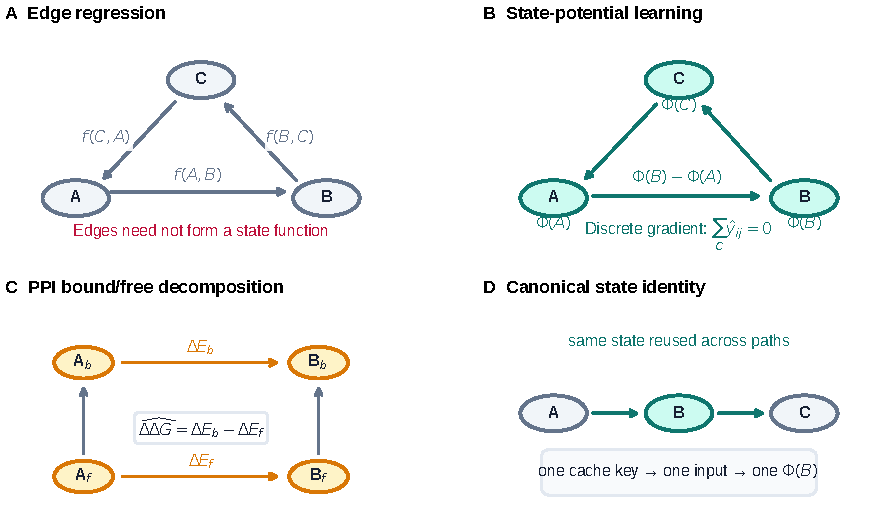
\includegraphics[width=\textwidth]{figures/fig1_state_potential_concept.pdf}
  \caption{DiMA-PPI reformulates the prediction target. (A) Independent edge regression assigns unrelated values to directed mutation pairs. (B) A shared potential assigns values to canonical mutation states and obtains every edge as a potential difference, producing a discrete gradient field. (C) For PPI binding, each mutation-state potential is decomposed into bound and free structural contexts. (D) Canonical caching makes an intermediate state identical wherever it occurs, which is necessary for algebraic path cancellation to survive the full computational pipeline.}
  \label{fig:state_potential_concept}
\end{figure}

\section{Related work}
\label{sec:related}

\noindent\textbf{Prediction of mutation-induced binding changes.}

Early structure-based approaches estimated energetic changes with physical or empirical energy functions. Computational alanine scanning provided an influential interface-energy formulation~\cite{kortemme2002}, while FoldX developed a widely used empirical force field for mutation effects~\cite{foldx}. Subsequent machine-learning methods combined structural environments with statistical potentials and evolutionary information. BeAtMuSiC uses coarse-grained statistical potentials~\cite{beatmusic}; SAAMBE combines sequence and structural descriptors~\cite{saambe}; and BindProfX incorporates interface profiles with a FoldX-based energy term~\cite{bindprofx}. Later predictors increased model and feature complexity: iSEE uses evolutionary and structure-derived features~\cite{isee}, mCSM-PPI2 represents mutation environments through graph-based signatures~\cite{mcsmpii2}, and MutaBind2 integrates interaction terms with machine learning for single and multiple mutations~\cite{mutabind2}. TopNetTree couples persistent-topology descriptors with ensemble learning~\cite{topnettree}.

Recent work has shifted toward learned sequence and geometric representations. GraphPPI introduced graph-based pretraining for mutation-effect prediction~\cite{graphppi}. MpbPPI combines multi-task pretraining with equivariant geometric learning~\cite{mpbppi}. RDE-Network models residue side-chain conformational distributions and learns energetic changes from structural environments~\cite{rdenetwork}. PPIFormer applies equivariant masked modeling to protein--protein interfaces and emphasizes leakage-resistant evaluation~\cite{ppiformer}. MuToN combines geometric learning with nonlocal residue communication~\cite{muton}. DSSA-PPI, our principal recent same-task accuracy reference, fuses ESM-2 and equivariant structural representations through disentangled structure--sequence attention and uses a residue-logit difference score~\cite{dssappi}. DiMA-PPI makes a distinct requirement: every mutation edge must be the difference of potentials assigned to canonical bound/free mutation states, independent of the edge-specific preprocessing path by which a state is reached.

These methods differ in training data, mutant-structure requirements, pretraining, and split construction. Consequently, results obtained under different random or complex-level partitions are not directly comparable. We therefore use the exact predefined S1129 evaluation folds distributed with DSSA-PPI~\cite{dssappi} and distinguish locally computed results from literature-reported baselines.

\medskip
\noindent\textbf{Physical consistency and state functions.}

The direct/reverse mutation relation provides a clear example of domain knowledge constraining model outputs. Many established $\ddg$ predictors produce biased and mutually inconsistent direct/reverse estimates, and post-hoc antisymmetrization can substantially change apparent accuracy~\cite{ddgbias}. DDMut-PPI uses forward and hypothetical reverse mutations in a Siamese construction~\cite{ddmutppi}, whereas DSSA-PPI guarantees pairwise antisymmetry through a difference of wild-type and mutant residue logits~\cite{dssappi}. JanusDDG, developed for protein stability rather than PPI binding, applies an antisymmetrized pairwise output and subsequently encourages transitivity with a dedicated fine-tuning loss~\cite{janusddg}. These studies establish the importance of thermodynamic relations; consequently, we do not claim to introduce antisymmetry or transitivity. The distinction of DiMA-PPI is the parameterization: one canonical potential is assigned to each mutation state and every edge is its discrete gradient. Pairwise antisymmetry, arbitrary-path additivity, and zero closed-loop circulation are therefore identities of the function class, rather than empirical effects of augmentation, output symmetrization, or a consistency loss. This connects knowledge-guided learning~\cite{pinnreview} to exact path independence, while retaining soft and hard pairwise variants as matched controls rather than as the proposed formulation.

\section{Materials and methods}
\label{sec:methods}

\subsection{Datasets and evaluation protocols}

The main study is restricted to single substitutions. We follow the DSSA-PPI sign convention: positive $\ddg$ denotes stronger mutant binding and negative $\ddg$ denotes weaker binding. The historical S1131 protocol contains 1,131 interface substitutions; after the two official 2I9B exclusions it yields 1,129 evaluable mutations from 111 complexes (hereafter S1129)~\cite{skempi1,skempi2,dssappi}. We use the predefined five complex-disjoint folds, containing 169, 142, 271, 252, and 295 test mutations. Original row indices, mutation strings, structures, labels, and fold membership were audited, and no official complex crosses folds.

Two complementary five-fold partitions probe distribution shift. For the sequence-aware partition, chains are clustered with MMseqs2 at 30\% identity and 80\% bidirectional coverage, complexes are connected when any constituent chains share a cluster, and connected components remain within folds~\cite{mmseqs2}. For the interface-aware partition, residues within 6~\AA{} of the partner define interface substructures, which are compared with US-align in multimer mode; connected structural groups remain within folds~\cite{usalign}. These partitions test different novelty axes and are not treated as an ordered difficulty ladder.

S4169, M1707, sequence-decontaminated AbBind, the c-MET laboratory panel, subgroup analyses, and the earlier soft/hard objective diagnostics are retained as secondary evidence in the Supplementary Material. They are not used to support the central state-potential claim. In particular, the main formulation and path audit do not claim multi-substitution epistasis.

\subsection{Canonical mutation-state construction}

A state is keyed by
\begin{equation}
  k=(\text{official complex},\text{chain},\text{PDB site},
  \text{amino-acid identity},\text{bound/free}).
  \label{eq:canonical_key}
\end{equation}
All records referring to the same key reuse one cached representation selected deterministically before fitting, without target or fold information. Canonicalization is essential when a wild-type state occurs in multiple mutation records: otherwise stochastic side-chain repacking can create edge-specific copies of the same state and destroy numerical path cancellation even when the network is written as a potential difference.

The original four-state cache contained 3,298 distinct state/context keys. Among 184 keys referenced more than once, 35 had nonidentical independently generated descriptors, with a maximum channel range of 11.083. After canonicalization, 1,218 repeated-state comparisons were identical element by element. The complete state input---sequence block, ProteinMPNN block, graph geometry and masks, and four-state descriptor---had maximum absolute difference zero, and no graph-structure mismatch was detected.

\subsection{Shared state encoder and four-state descriptors}

Residues within 20~\AA{} of the substitution form a local graph. Residues within 8~\AA{} are connected, with sequential covalent neighbors retained, and edge distances are expanded with 16 radial basis functions. Each state supplies residue-level ESM-2 650M embeddings and a ProteinMPNN representation of the reference backbone~\cite{esm2,proteinmpnn}. Mutated-chain, partner-chain, mutation-site, and normalized-distance indicators are appended. Separate sequence and structure projections are combined by a learned gate,
\begin{align}
 h_i^{\mathrm{seq}} &= \phi_{\mathrm{seq}}(x_i^{\mathrm{seq}}), \\
 h_i^{\mathrm{str}} &= \phi_{\mathrm{str}}(x_i^{\mathrm{str}}), \\
 g_i &= \sigma\!\left(W_g[h_i^{\mathrm{seq}},h_i^{\mathrm{str}},s_i]\right), \\
 h_i &= \mathrm{LN}\!\left(h_i^{\mathrm{seq}}+g_i\odot h_i^{\mathrm{str}}+W_s s_i\right).
\end{align}
Three four-head TransformerConv layers propagate local information. Attention pooling returns a mutation-site representation and a contextual representation. For a free state, partner-chain nodes and cross-chain edges are excluded from message passing and readout; for a bound state, both partners are retained.

The explicit state descriptor is computed for wild-type bound, mutant bound, wild-type free, and mutant free states in that order. The source complex is loaded in PyRosetta. Wild-type and mutant bound poses are independently side-chain repacked within 8~\AA{} of the site; the mutated chain is also isolated and repacked to construct the two free states. Each 141-dimensional descriptor contains same-chain and partner-chain element-distance histograms, mutated-residue element counts, 18 residue Rosetta score terms, and the same 18 terms summed over the local environment. These are computational structural hypotheses, not experimentally resolved mutant structures or fully relaxed ensembles. In particular, the isolated-chain free context is not an equilibrium estimate of the physical unbound ensemble or its absolute free energy. Persistent topology and the old pairwise mutant-minus-wild-type atomic-delta branch are not used by the state-potential forward path.

\subsection{Thermodynamically integrable state-potential learning}

One shared network $E_\theta$ evaluates all four state/context combinations. For an amino-acid state $S$, define
\begin{equation}
  \Phi_\theta(S)=E_\theta(S_{\mathrm{bound}})-E_\theta(S_{\mathrm{free}}).
  \label{eq:binding_potential}
\end{equation}
The predicted effect of replacing $A$ by $B$ is
\begin{align}
 \widehat{\ddg}_{A\rightarrow B}
 &=\left[E_\theta(B_{\mathrm{bound}})-E_\theta(A_{\mathrm{bound}})\right]
   -\left[E_\theta(B_{\mathrm{free}})-E_\theta(A_{\mathrm{free}})\right] \\
 &=\Phi_\theta(B)-\Phi_\theta(A).
 \label{eq:four_state_cycle}
\end{align}

\noindent\textbf{Proposition (exact integrability).}
If every mutation edge is parameterized as
$\widehat{y}_{ij}=\Phi_\theta(j)-\Phi_\theta(i)$ using one shared potential
over canonical states, then for any states $i,j,k$,
\begin{align}
 \widehat{y}_{ij}&=-\widehat{y}_{ji},\\
 \widehat{y}_{ik}&=\widehat{y}_{ij}+\widehat{y}_{jk},
 \label{eq:exact_properties}
\end{align}
and for every closed cycle $C$,
\begin{equation}
 \sum_{(i,j)\in C}\widehat{y}_{ij}=0.
 \label{eq:closed_cycle}
\end{equation}
\textit{Proof.} Substituting the potential difference makes the reverse and
three-state identities immediate; summing around a closed cycle telescopes,
so every potential appears once with each sign. \hfill$\square$

The model is trained only with Smooth-L1 loss on observed forward $\ddg$
values; no reverse label, consistency penalty, or $\lambda_{\mathrm{anti}}$ is
used.

Individual $E_\theta$ and $\Phi_\theta$ values are not uniquely identifiable. Additive gauge transformations can leave every observed difference unchanged, and supervision is available only through binding effects. We therefore interpret them as latent computational potentials, not absolute physical free energies.

\subsection{Matched controls and real mutation-path audit}

We compare the proposed model with an unconstrained pairwise regressor, reverse-label supervision, soft consistency, hard pairwise antisymmetry, and a shared-potential control without the explicit four-state descriptors. Soft consistency uses the fixed weight 0.20 only as a historical mechanism control; it is not the primary model and is not used to select the state-potential architecture. The hard control computes $[f(A,B)-f(B,A)]/2$, guaranteeing Eq.~\eqref{eq:physical_antisymmetry} but not Eq.~\eqref{eq:path_additivity}.

For the path audit, we identify held-out sites with at least two experimentally assayed mutant endpoints. The 92 resulting panels contain 4,952 unordered mutant pairs and 9,904 ordered paths $A\rightarrow B\rightarrow C$. Every panel is evaluated by the outer-fold model that excluded its complete complex. The intermediate $B\rightarrow C$ edge is constructed from real assayed endpoint states but has no independent experimental label; the audit measures internal integrability, not $B\rightarrow C$ predictive accuracy. To define this edge fairly for all models, matched path controls use the common ESM-2, ProteinMPNN, and residue-graph inputs but omit directional atomic deltas and topology, neither of which has a unique observed $B\rightarrow C$ value. The four prespecified models are the pairwise backbone, soft consistency, hard pairwise antisymmetry, and the canonical state potential. We define
\begin{equation}
 \epsilon_{\mathrm{path}}=
 \left|\widehat{\ddg}_{A\rightarrow C}
 -\widehat{\ddg}_{A\rightarrow B}
 -\widehat{\ddg}_{B\rightarrow C}\right|,
\end{equation}
and $\epsilon_{\mathrm{rev}}=|\widehat{\ddg}_{A\rightarrow B}+\widehat{\ddg}_{B\rightarrow A}|$. In addition, all state subsets generate 31,922 deterministic triangle cycles and 133,736 four-state cycles per model. One canonical orientation per subset is fixed from source-row order before prediction, and circulation is the absolute sum of the directed edge predictions around the closed loop. We report the mean, median, 95th percentile, maximum, and fractions below 0.1 and $10^{-3}$~kcal mol$^{-1}$ for every error. The structural audit uses the prespecified representative seed 43 because exactness of the state-potential construction is seed independent; main predictive comparisons use all five seeds.

\subsection{Training and evaluation}

Models use a hidden dimension of 96, three graph layers, dropout 0.15, AdamW with learning rate $5\times10^{-4}$ and weight decay $10^{-4}$, batch size 8, and SmoothL1 $\beta=0.5$. Approximately one eighth of each outer training fold is assigned by a seeded mutation-level split to validation and used for MSE-based early stopping. Thus, outer test folds are strictly complex disjoint, whereas the inner early-stopping split is not complex grouped. Training runs for at most 60 epochs with patience 10. Target scaling uses the fitting subset and fixes the mean at zero for potential-difference and hard-antisymmetric models so that transformation back to kcal mol$^{-1}$ preserves exactness.

Pearson correlation on S1129 is the primary metric; Spearman correlation, RMSE, MAE, and AUROC are complementary. Main predictive comparisons use seeds 42--46. Tables report mean and sample standard deviation across seeds after averaging fold metrics within each seed. The DSSA-PPI comparison uses the same 1,129 observations, public outer-fold assignments, labels, and fold-mean metric definition. It remains descriptive because training, pretraining, inputs, optimization, and per-mutation baseline predictions are not matched or available for paired testing.

For paired uncertainty analysis, predictions are first averaged across seeds. The primary bootstrap resamples whole official complexes independently within each outer fold 10,000 times, computes each metric in every fold, and averages the five fold metrics. Because correlation is nonlinear, this five-seed ensemble estimand need not equal the difference between seed-wise means in a table. Sequence- and interface-aware results use complex-grouped bootstrap. Intervals that cross zero are described as numerical rather than statistically supported changes.

\section{Results}
\label{sec:results}

\subsection{Performance on unseen protein complexes}

The first question is whether exact integrability preserves competitive accuracy on the primary unseen-complex task. On the predefined S1129 folds, the canonical state-potential model achieved $0.757\pm0.009$ Pearson correlation and $0.799\pm0.006$ AUROC (Table~\ref{tab:baselines}). These values are numerically higher than the reported DSSA-PPI result ($0.71\pm0.01$ and $0.77\pm0.02$, respectively). DSSA-PPI is the principal same-task accuracy reference because it is a recent structure--sequence predictor evaluated on the same observations and outer folds. Nevertheless, this is a descriptive protocol-aligned comparison, not evidence of paired statistical superiority: the methods differ in pretraining, inputs, optimization, and training procedure, and DSSA-PPI per-mutation predictions are unavailable.

\begin{table}[t]
\centering
\caption{Performance on the official S1129 unseen-complex folds. Baselines are values reported by DSSA-PPI for the same observations, outer folds, and fold-mean metric definition; ours is locally computed. Training pipelines and per-mutation predictions are not matched, so cross-method differences are descriptive rather than paired comparisons.}
\label{tab:baselines}
\resizebox{\textwidth}{!}{%
\begin{tabular}{lccc}
\toprule
Method & Pearson & AUROC & Provenance \\
\midrule
FoldX~\cite{foldx} & 0.44 & 0.70 & Reported \\
MpbPPI~\cite{mpbppi} & $0.48\pm0.04$ & $0.75\pm0.02$ & Reported \\
PPIFormer~\cite{ppiformer} & $0.68\pm0.01$ & $0.72\pm0.02$ & Reported \\
MuToN~\cite{muton} & $0.70\pm0.01$ & $0.74\pm0.01$ & Reported \\
DSSA-PPI~\cite{dssappi} & $0.71\pm0.01$ & $0.77\pm0.02$ & Reported \\
DiMA-PPI (canonical state potential) & $\mathbf{0.757\pm0.009}$ & $\mathbf{0.799\pm0.006}$ & Local \\
\bottomrule
\end{tabular}
}
\end{table}

DDMut-PPI is retained as an established PPI mutation baseline and reported
PCC values up to approximately 0.75 with RMSE 1.33~kcal mol$^{-1}$ under its
own leave-one-complex-out evaluation~\cite{ddmutppi}. Because its observation
cohort and evaluation construction are not the official S1129 five folds, we
do not insert that number into Table~\ref{tab:baselines} or treat it as a
direct numerical ranking.

\subsection{Changing the hypothesis class while retaining predictive accuracy}
\label{sec:predictive_value}

The controlled comparison in Table~\ref{tab:model_comparison} separates the proposed parameterization from earlier ways of injecting the reverse relation. All rows use the same official folds, graph backbone, optimization schedule, and seeds. The unconstrained pairwise regressor reached $0.570\pm0.020$ PCC. Reverse-label supervision, soft consistency, and hard antisymmetry all increased PCC to approximately 0.75, confirming that directional structure is highly informative on this benchmark. The canonical four-state potential reached $0.757\pm0.009$ PCC and the lowest mean RMSE and MAE, despite using neither reverse labels nor a consistency coefficient. Its performance was comparable to the soft and hard controls; the small differences among these three rows do not establish predictive superiority of one constraint mechanism.

\begin{table}[t]
\centering
\caption{Matched model comparison on the official S1129 unseen-complex folds. Values are mean $\pm$ standard deviation over seeds 42--46 after averaging fold metrics within each seed. The state-potential models have no antisymmetry coefficient.}
\label{tab:model_comparison}
\resizebox{\textwidth}{!}{%
\begin{tabular}{lcccc}
\toprule
Model & Pearson & Spearman & RMSE & MAE \\
\midrule
Unconstrained pairwise & $0.5699\pm0.0202$ & $0.5140\pm0.0206$ & $2.1116\pm0.0471$ & $1.3949\pm0.0342$ \\
Reverse-label supervision & $0.7563\pm0.0093$ & $0.6021\pm0.0108$ & $1.5651\pm0.0389$ & $1.1933\pm0.0328$ \\
Soft consistency & $\mathbf{0.7592\pm0.0124}$ & $\mathbf{0.6076\pm0.0137}$ & $1.5510\pm0.0446$ & $1.1708\pm0.0455$ \\
Hard pairwise antisymmetry & $0.7546\pm0.0025$ & $0.5940\pm0.0087$ & $1.5494\pm0.0128$ & $1.1674\pm0.0068$ \\
Shared potential, no state descriptors & $0.7497\pm0.0044$ & $0.5784\pm0.0063$ & $1.5883\pm0.0245$ & $1.1799\pm0.0198$ \\
Canonical four-state potential & $0.7574\pm0.0094$ & $0.5918\pm0.0112$ & $\mathbf{1.5415\pm0.0230}$ & $\mathbf{1.1605\pm0.0151}$ \\
\bottomrule
\end{tabular}}
\end{table}

The no-state shared-potential row is the decisive control for the PPI-specific bound/free descriptors. In the five-seed ensemble, adding four-state descriptors changed fold-mean PCC by $+0.0098$ (95\% CI 0.0002--0.0206) and RMSE by $-0.0490$~kcal mol$^{-1}$ ($-0.0779$ to $-0.0138$); both intervals excluded zero. MAE changed by $-0.0172$~kcal mol$^{-1}$ ($-0.0427$ to 0.0149), so that reduction is numerical only. Figure~\ref{fig:predictive_value} visualizes both the matched models and this paired comparison. The ensemble bootstrap values differ slightly from differences between seed-wise table means because predictions are first averaged across seeds and nonlinear metrics are then computed within each fold.

\begin{figure}[t]
  \centering
  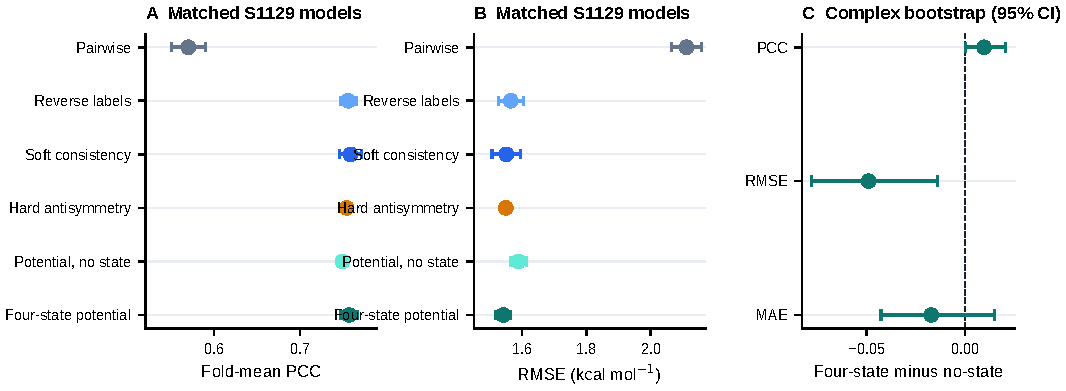
\includegraphics[width=\textwidth]{figures/fig3_predictive_value.pdf}
  \caption{Predictive value of the state-potential formulation on S1129. (A,B) Five-seed fold-mean PCC and RMSE for matched pairwise, consistency, and shared-potential models. Error bars are standard deviations across seeds. (C) Four-state minus no-state shared-potential differences from a 10,000-replicate fold-stratified complex bootstrap of five-seed ensemble predictions. Bars are 95\% confidence intervals; positive PCC and negative error differences favor the four-state model.}
  \label{fig:predictive_value}
\end{figure}

\subsection{Exact antisymmetry is insufficient for integrability}
\label{sec:integrability_results}

The path audit provides the central mechanism test. Across 92 held-out mutation panels, it evaluates 5,653 reverse comparisons, 9,904 ordered three-state paths, 31,922 triangle cycles, and 133,736 four-state cycles. Pairwise regression had large errors for every relation, whereas soft consistency reduced but did not eliminate them (Table~\ref{tab:integrability}). Hard antisymmetry reduced mean reverse error to $1.18\times10^{-7}$~kcal mol$^{-1}$, yet its mean three-state path error remained 0.417~kcal mol$^{-1}$ and its mean four-state circulation remained 0.315~kcal mol$^{-1}$. Thus, numerical satisfaction of the reverse identity does not imply the existence of a shared state function.

In contrast, the canonical state-potential model reduced the mean reverse, path, triangle-cycle, and four-state-cycle errors to $1.84\times10^{-7}$, $3.12\times10^{-7}$, $2.50\times10^{-7}$, and $2.91\times10^{-7}$~kcal mol$^{-1}$, respectively. Every tested relation was below $10^{-3}$~kcal mol$^{-1}$. These residuals are floating-point effects rather than learned approximations and confirm that both the parameterization and the cached implementation preserve exact integrability (Fig.~\ref{fig:integrability_audit}). The audit does not test the accuracy of the constructed $B\rightarrow C$ edge, for which no independent experimental label exists; it tests whether predictions over real assayed endpoint states form a path-independent field.

\begin{table}[t]
\centering
\caption{Held-out real-state integrability audit. Entries are mean absolute error with the 95th percentile in parentheses, in kcal mol$^{-1}$. Full medians, maxima, and threshold fractions are reported in Supplementary Table~S2.}
\label{tab:integrability}
\resizebox{\textwidth}{!}{%
\begin{tabular}{lccc}
\toprule
Model & Reverse error & Three-state path error & Four-state circulation \\
\midrule
Pairwise & 2.295 (5.540) & 1.333 (3.537) & 4.209 (10.335) \\
Soft consistency & 0.892 (2.746) & 0.920 (2.952) & 1.709 (5.292) \\
Hard pairwise antisymmetry & $1.18\!\times\!10^{-7}$ ($4.77\!\times\!10^{-7}$) & 0.417 (1.478) & 0.315 (1.078) \\
Canonical state potential & $1.84\!\times\!10^{-7}$ ($5.96\!\times\!10^{-7}$) & $3.12\!\times\!10^{-7}$ ($1.06\!\times\!10^{-6}$) & $2.91\!\times\!10^{-7}$ ($8.59\!\times\!10^{-7}$) \\
\bottomrule
\end{tabular}}
\end{table}

\begin{figure}[t]
  \centering
  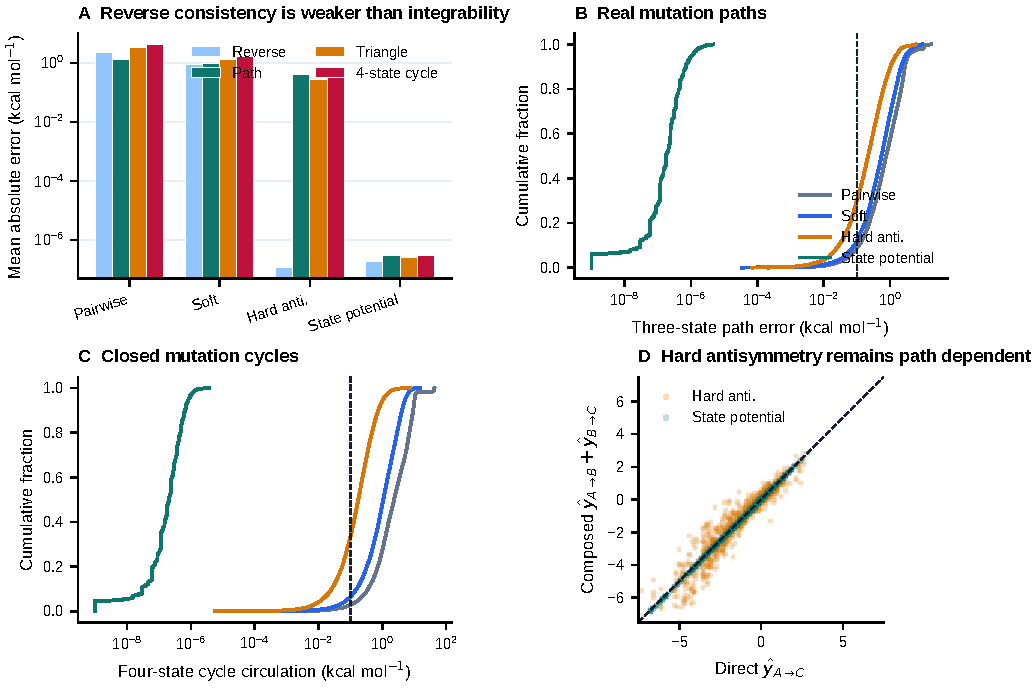
\includegraphics[width=\textwidth]{figures/fig2_integrability_audit.pdf}
  \caption{Antisymmetry versus thermodynamic integrability. (A) Mean reverse, path, triangle-cycle, and four-state-cycle errors on a logarithmic scale. (B,C) Empirical cumulative distributions for 9,904 real-state paths and 133,736 four-state cycles; dashed lines mark 0.1~kcal mol$^{-1}$. (D) Direct versus composed predictions for the hard-antisymmetric and state-potential models. Hard antisymmetry lies off the identity line despite near-zero reverse error, whereas state-potential predictions cancel to numerical precision.}
  \label{fig:integrability_audit}
\end{figure}

\subsection{Generalization under distinct distribution shifts}

Sequence- and interface-aware partitions probe complementary forms of distribution shift rather than successive levels of one ordered hierarchy. Absolute performance decreased substantially relative to the official unseen-complex folds for every model (Table~\ref{tab:strict_results}). On the sequence-cluster split, the state potential reached PCC 0.354 and RMSE 2.355~kcal mol$^{-1}$; on the interface-structure split it reached PCC 0.488 and RMSE 2.174~kcal mol$^{-1}$. The corresponding soft and hard controls were similar in scale.

Complex-grouped paired bootstrap provides no statistically supported state-potential improvement or degradation in the main regression metrics. For sequence shift, state-potential minus backbone PCC was $+0.012$ (95\% CI $-0.180$ to 0.183), while state-potential minus soft and hard PCC were $-0.027$ ($-0.204$ to 0.116) and $-0.038$ ($-0.154$ to 0.056). For interface shift, the three PCC differences were $+0.019$ ($-0.071$ to 0.129), $-0.002$ ($-0.058$ to 0.053), and $+0.025$ ($-0.011$ to 0.065), respectively. RMSE and MAE intervals likewise crossed zero for all three matched contrasts in both shifts. Therefore exact integrability preserves an exact physical structure under distribution shift, but the present data do not support a claim that it improves remote sequence or interface extrapolation.

\begin{table}[t]
\centering
\caption{Five-seed ensemble results under sequence- and interface-aware partitions. These shifts are parallel evaluation axes, not an ordered difficulty ladder.}
\label{tab:strict_results}
\resizebox{\textwidth}{!}{%
\begin{tabular}{llrrrr}
\toprule
Split & Model & Pearson & Spearman & RMSE & MAE \\
\midrule
\multirow{4}{*}{Sequence cluster}
& Unconstrained backbone & 0.341 & 0.431 & 2.290 & 1.520 \\
& Soft consistency & 0.380 & 0.451 & 2.252 & 1.502 \\
& Hard pairwise antisymmetry & \textbf{0.392} & \textbf{0.475} & \textbf{2.257} & \textbf{1.487} \\
& Canonical state potential & 0.354 & 0.441 & 2.355 & 1.519 \\
\midrule
\multirow{4}{*}{Interface structure}
& Unconstrained backbone & 0.469 & 0.547 & 2.163 & 1.451 \\
& Soft consistency & \textbf{0.490} & \textbf{0.552} & \textbf{2.136} & \textbf{1.421} \\
& Hard pairwise antisymmetry & 0.463 & 0.509 & 2.194 & 1.463 \\
& Canonical state potential & 0.488 & 0.515 & 2.174 & 1.458 \\
\bottomrule
\end{tabular}}
\end{table}

\begin{figure}[t]
  \centering
  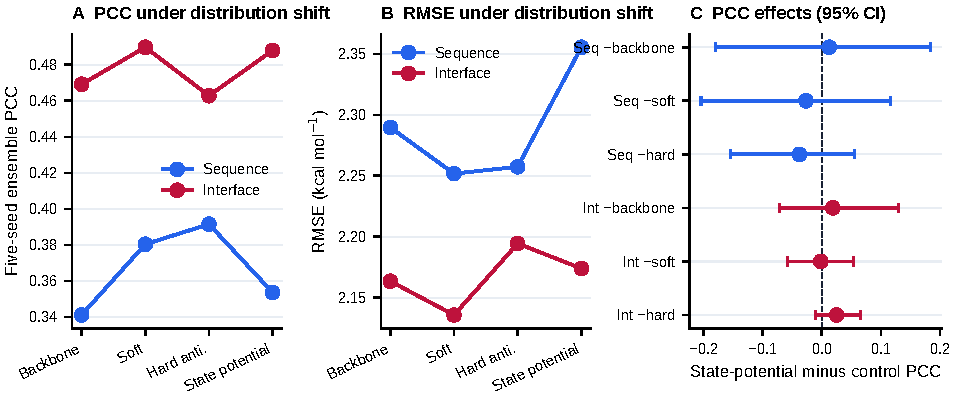
\includegraphics[width=\textwidth]{figures/fig4_strict_boundary.pdf}
  \caption{Boundary under distinct distribution shifts. (A,B) Five-seed ensemble PCC and RMSE for matched models on sequence-cluster and interface-structure partitions. (C) State-potential minus control PCC with 95\% complex-bootstrap intervals. Every interval crosses zero. The two partitions represent different novelty axes and are not presented as an ordered strictness ladder.}
  \label{fig:strict_boundary}
\end{figure}

External transfer to 395 sequence-decontaminated AbBind mutations likewise provided no statistically supported model difference (Supplementary Table~S4). This is consistent with the strict-split result: an exact state-function structure prevents thermodynamic contradictions, but it cannot recover missing interaction context or training coverage.

\subsection{Secondary analyses}

Additional benchmarks and historical pairwise-constraint analyses are reported separately so that they do not obscure the state-potential evidence chain. S4169 and M1707 results use different retained cohorts and preprocessing variants and are therefore descriptive rather than controlled comparisons with DSSA-PPI. Exploratory subgroup, feature, reverse-direction, case-study, and c-MET analyses likewise concern the earlier pairwise soft/hard models rather than the canonical state-potential formulation. They are retained in the Supplementary Material for transparency but do not support the central integrability claim.

Two observations remain relevant to scope. First, removing persistent-topology descriptors from the earlier pairwise model did not reduce accuracy; topology is consequently absent from the state-potential forward path and is not presented as an innovation. Second, the c-MET sequence-only stress test showed that physical self-consistency can improve while external ranking does not. This negative result complements the strict-split analysis by separating thermodynamic admissibility from predictive validity under missing interaction structure.

\section{Discussion}
\label{sec:discussion}

The main contribution of DiMA-PPI is representational rather than a claim of universal accuracy improvement. Standard models learn mutation edges, even when reverse labels or antisymmetric outputs constrain selected relations. DiMA-PPI instead learns canonical mutation states and obtains every mutation effect as their potential difference. This restricts the admissible hypothesis class to discrete gradient fields. The resulting reverse relation, arbitrary-path additivity, and zero cycle circulation are not empirical tendencies that require successful optimization; they are identities of every function the model can represent.

The path audit makes the distinction from hard antisymmetry concrete. A hard pairwise model can assign $f(A,B)=-f(B,A)$ to every edge while the independently predicted edges $A\rightarrow B$, $B\rightarrow C$, and $A\rightarrow C$ fail to telescope. This is exactly what we observe: reverse error is at floating-point precision, but mean path error remains 0.417~kcal mol$^{-1}$. DiMA-PPI reduces both quantities, as well as triangle and four-state circulation, to numerical precision. Consequently, the closest conceptual comparison is not whether DiMA-PPI has a smaller reverse error than another exactly antisymmetric method; it is whether the model represents an integrable state function rather than an antisymmetric edge field.

The bound/free construction adds a PPI-specific layer to this general principle. A mutation can alter both the complex and the isolated partner, so a binding effect is naturally expressed as a difference between bound and free mutation responses. The paired no-state control indicates that explicit four-state descriptors contribute a small but supported improvement in PCC and RMSE on S1129. This evidence argues that the decomposition is not merely decorative. It does not, however, establish that the latent $E_\theta$ values are calibrated physical free energies. Only their supervised differences are identifiable, and the isolated-chain computational context is an approximation rather than an equilibrium unbound ensemble.

The strict partitions define the boundary of the present evidence. All models lose substantial accuracy under sequence and interface novelty, and the state-potential differences from pairwise, soft, and hard controls are statistically unsupported for the main regression metrics. Exact integrability therefore solves a consistency problem, not the broader extrapolation problem. The result also cautions against equating a physical guarantee with improved distributional robustness: a model can remain exactly integrable while its learned state potentials are inaccurate outside the training distribution.

Canonical state identity is an implementation requirement with methodological consequences. Before canonicalization, independently repacked copies of the same nominal state differed in 35 of 184 repeated keys, making path cancellation input dependent. Reusing one deterministic representation per complex, site, residue identity, and context closes this gap between the algebraic definition and the actual inference pipeline. Canonicalization should therefore accompany any state-potential model whose preprocessing is stochastic or edge specific.

Several limitations remain. The study formally models single substitutions; multi-site epistasis would require a state definition and sampling design beyond the present work. The path audit uses real assayed endpoint states, but intermediate mutant-to-mutant edges lack independent experimental labels, so it demonstrates internal integrability rather than their predictive accuracy. Repacked static structures do not capture large conformational changes, solvent and protonation effects, or full unbound ensembles. The latent potentials are gauge dependent and must not be interpreted as absolute free energies. Literature comparisons, including DSSA-PPI, remain descriptive because training and pretraining pipelines differ and paired predictions are unavailable. Finally, preprocessing with ESM-2, ProteinMPNN, and PyRosetta is materially more expensive than the loaded-feature network pass, and the strict-split confidence intervals remain wide. Future work should evaluate integrable state learning with larger mutation panels, independently measured multi-step paths, conformational ensembles, and broader complex families.

\section{Conclusion}
\label{sec:conclusion}

DiMA-PPI reformulates mutation-induced PPI binding prediction from independent edge-wise $\ddg$ regression into shared latent potential learning over canonical mutation states. Defining mutation effects as differences of bound/free state potentials restricts predictions to a discrete gradient field, so reverse antisymmetry, arbitrary-path additivity, and zero closed-cycle circulation are exact properties of the model function class. The held-out audit shows why this is stronger than hard antisymmetry: near-zero reverse error can coexist with substantial path error, whereas the state-potential model satisfies both to numerical precision.

This stronger thermodynamic structure retains competitive accuracy on the primary S1129 unseen-complex benchmark, and the four-state descriptors provide supported PCC and RMSE gains over a no-state potential control. It does not, by itself, improve prediction under stronger sequence or interface shifts. The appropriate conclusion is therefore not that integrability universally improves generalization, but that it defines a physically admissible and empirically competitive mutation predictor whose guarantees are exact, interpretable, and separable from predictive accuracy.

\section*{Declaration of competing interest}
The authors declare that they have no known competing financial interests or personal relationships that could have appeared to influence the work reported in this paper.

\section*{Data availability}
SKEMPI~2.0 and the DSSA-PPI benchmark folds are publicly available from their original sources. The normalized c-MET measurements, full wild-type and mutant sequences, processed split definitions, leakage audits, summary tables, OOF predictions, analysis scripts, figure-generation code, and run configurations used in this study are supplied in a machine-readable reproducibility archive with the manuscript. The archive is available to editors and reviewers during peer review and will be deposited in a permanent public repository upon publication.

\section*{Declaration of generative AI and AI-assisted technologies in the manuscript preparation process}
During the preparation of this work, the authors used OpenAI Codex to improve language, clarity, and manuscript organization and to assist with reference-format checks. After using this service, the authors reviewed and edited the content as needed and take full responsibility for the content of the published article.

\bibliographystyle{elsarticle-num}
\bibliography{kbs_references}

\end{document}
